% Kapitel 3
%-------------------------------------------------------------------------------
\chapter{Produktübersicht}

\begin{figure}[h]
\centering
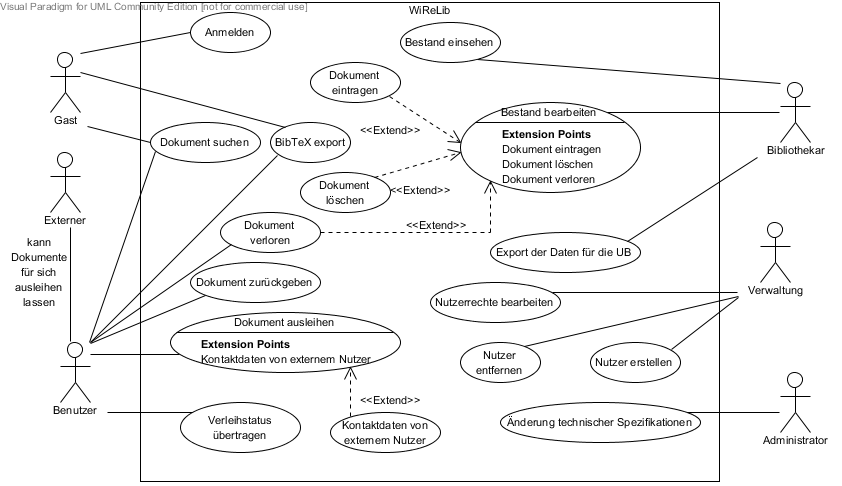
\includegraphics[width=0.8\linewidth]{bilder/use-case.png}
\caption[Use-Case-Diagramm]{Use-Case-Diagramm}
\label{use-case}
\end{figure}

Details zur Abbildung \ref{use-case} \nameref{use-case}  werden folgend beschrieben.

Benutzer, die nicht angemeldet sind, werden als Gäste geführt.
Gäste können sich anmelden und sind dann Nutzer.
Auch können Gäste Dokumente suchen und herausfinden, ob sie vorhanden sind, oder ob sie bereits verliehen wurden.

Ein Nutzer darf wie ein Gast nach Dokumenten suchen.
Zusätzlich darf er Dokumente ausleihen und muss diese auch wieder zurückgeben.
Wenn ihm ein Dokument verloren geht, sollte er dies melden.
Auch darf ein Nutzer ein ausgeliehenes Dokument weitergeben.
Dabei wird der Verleihstatus auf die andere Person übertragen.
Wenn dies \gls{glos:ext}\ sind, so müssen die Kontaktdaten hinterlegt werden.

Der Bibliothekar kann den Bestand der Dokumente einsehen und ihn bearbeiten.
Das heißt, dass er neue Dokumente eintragen kann, aus der Suchoption entfernen, oder ein Dokument als verloren markieren, sodass, falls möglich, neu bestellt werden kann.
Der Bibliothekar kann durch einen Button eine Datei exportieren, welche für die \gls{UB} lesbar ist.
Somit kann auch von der \gls{UB} aus ein gesuchtes Dokument gefunden werden.

Die Verwaltung darf Nutzer erstellen, Nutzerrechte bearbeiten und gegebenenfalls Nutzer entfernen.

Der Administrator hat vollen Zugriff auf das System und kann alle technische Spezifikationen vornehmen.
